\section{Aktive Filter} 

\subsection{Sallen-Key-Filter (Einfachmitkopplung)}

\begin{minipage}[c]{0.4\columnwidth}
    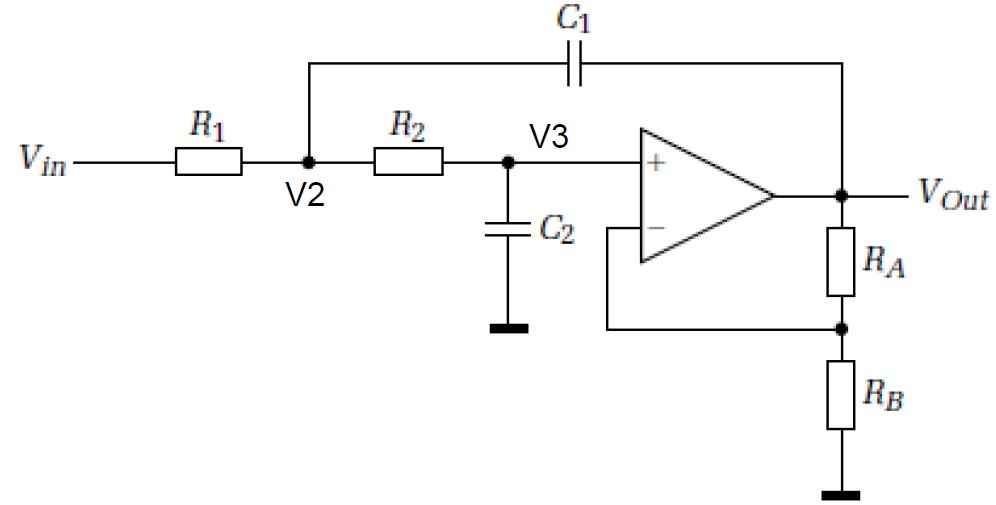
\includegraphics[width=\columnwidth]{images/sallen_key.png}
\end{minipage}
\hfill
\begin{minipage}[c]{0.58\columnwidth}
    $$ \text{OpAmp:} \quad  V_{\rm out} = G_0 \cdot V_3 = \Big(1 + \frac{R_A}{R_B} \Big) \cdot V_3 $$
    $$ \omega_0 = \frac{1}{\sqrt{C_1 C_2 R_1 R_2}} $$
    $$ Q = \frac{\sqrt{C_1 C_2 R_1 R_2}}{ C_2 (R_1 + R_2) + C_1 R_1 \cdot (1 - G_0)} $$
\end{minipage}

$$ \boxed{ G(s) = \frac{G_0}{ C_1 C_2 R_1 R_2 \cdot s^2 + [ C_2 (R_1 + R_2) + C_1 R_1 (1 - G_0) ] \cdot s + 1} } $$

\textbf{Stromgleichungen:}
\begin{align*}
    \text{V2:} \quad 0 &= (V_2 - V_{\rm in}) \frac{1}{R_1} + (V_2 - V_3) \frac{1}{R_2} + (V_2 - V_{\rm out}) \cdot s \cdot C_1  \\
    \text{V3:} \quad 0 &= (V_3 - V_2) \frac{1}{R_2} + V_3  \cdot s \cdot C_2 
\end{align*}


\subsubsection{Sallen-Key-Filter bei hohen Frequenzen}

\begin{minipage}[c]{0.4\columnwidth}  
    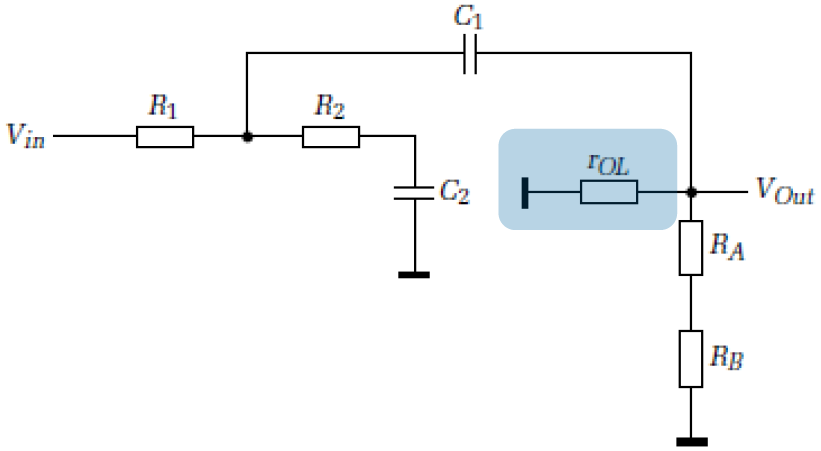
\includegraphics[width=\columnwidth]{images/sallen_key_hohe_frequenzen.png}
\end{minipage}
\hfill
\begin{minipage}[c]{0.58\columnwidth}
    $$ \boxed{ \frac{V_{\rm out}}{V_{\rm in}} \approx \frac{r_{\rm OL}}{R_1 + r_{\rm OL}} }$$
    $r_{\rm OL}$ ist der OpAmp open-loop Ausgangswiderstand (bei hohen Frequenzen $\approx 100 \, \ohm$)
\end{minipage}

\begin{itemize}
    \item Dämpfung ist limitiert auf obigen Spannungsteiler
        \textrightarrow\ Sallen-Key-Filter sind nicht geeignet für Systeme mit hohen Frequenzanteilen z.B. PWM-DAC
\end{itemize}


\subsection{Multiple-Feedback-Struktur}

\begin{minipage}[c]{0.4\columnwidth}
    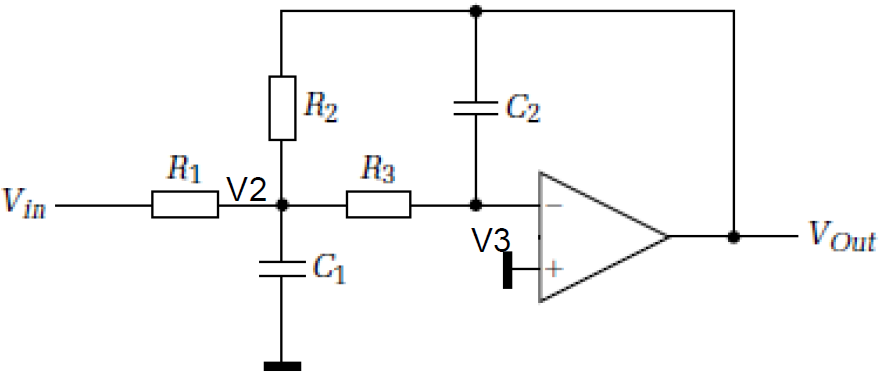
\includegraphics[width=\columnwidth]{images/aktive_filter_multiple_feedback.png}
\end{minipage}
\hfill
\begin{minipage}[c]{0.58\columnwidth}
    $$ \text{OpAmp:} \quad  G_0 = -\frac{R_2}{R_1} $$
    $$ Q = \frac{\sqrt{C_1 C_2 R_1 R_2}}{ C_2 \Big( R_2 + R_2 + R_3 \frac{R_2}{R_1} \Big)} $$
\end{minipage}

$$ \boxed{ G(s) = \frac{G_0}{1 + C_2 \Big( R_2 + R_2 + R_3 \frac{R_2}{R_1} \Big) \cdot s + C_1 C_2 R_2 R_3 \cdot s^2 }}$$

\textbf{Stromgleichungen:}
\begin{align*}
    \text{V2:} \quad 0 &= (V_2 - V_{\rm in}) \frac{1}{R_1} + (V_2 - V_{\rm out}) \frac{1}{R_2} + (V_2 - V_3) \frac{1}{R_3} + V_2 \cdot s \cdot C_1  \\
    \text{V3:} \quad 0 &= (V_3 - V_2) \frac{1}{R_3} + (V_3 - V_{\rm out})  \cdot s \cdot C_2 
\end{align*}


\subsection{Sallen-Key vs. Multiple-Feedback Struktur}

\begin{minipage}[t]{0.48\columnwidth}
    \begin{center}
        \myul{\textbf{Sallen-Key}}
    \end{center}
    \begin{outline}
        \1 Nicht-invertierend
        \1 $Q$ sensitiver auf Toleranzen
        \1 Vorwärtspfad für hohe Frequenzen
        \1 Noise-Gain: $A$
        \1 Eher für 
            \2 Hochpass
            \2 kleine Verstärkungen
    \end{outline}
\end{minipage}
\hfill
\begin{minipage}[t]{0.48\columnwidth}
    \begin{center}
        \myul{\textbf{Multiple-Feedback}}
    \end{center}
    \begin{outline}
        \1 Invertierend
        \1 $f_g$ sensitiver auf Toleranzen 
        \1[] 
        \1 Noise-Gain: $A+1$
        \1 Eher für 
            \2 Tiefpass, Bandpass
            \2 grössere Verstärkungen
    \end{outline}
\end{minipage}


\subsection{Vorgehen: UTF aus OPV-Filterschaltung ermitteln}
\begin{itemize}
    \item Stromgleichungen (Knotengleichungen) aufstellen
    \item Gleichungen ineinander einsetzen
    \item Umformen nach $G(s) = \frac{V_{\rm out}}{V_{\rm in}}$
\end{itemize}


\subsection{Zustandsvariablen-Filter (Biquad-Filter)}
\label{zustandsvariablenfilter}

\begin{minipage}[c]{0.6\columnwidth}
    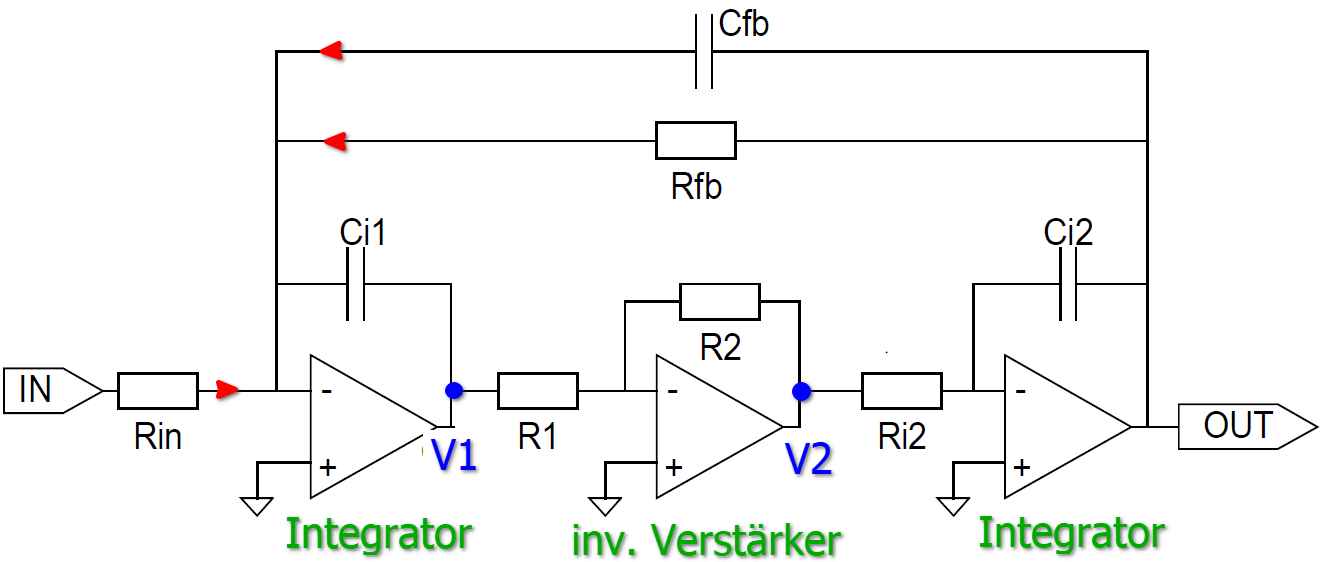
\includegraphics[width=\columnwidth]{images/zustandsvariablenfilter.png}
\end{minipage}
\hfill
\begin{minipage}[c]{0.38\columnwidth}
    \raggedright%
    Mit dieser Topologie sind alle drei \textbf{Parameter} $f_0$, $Q$ und $A_0$ \textbf{frei wählbar!} \\
    An $V_{\rm out}$ herrscht \textbf{Tiefpass-Verhalten.}
\end{minipage}

$$ \boxed{ G(s) = \frac{- \frac{R_{\rm fb}}{R_{\rm in}}}{s^2 \cdot C_{i1} C_{i2} R_{\rm fb} R_{i2} \frac{R_1}{R_2} + s \cdot C_{\rm fb} R_{\rm fb} + 1} } $$

$$ f_0 = \frac{1}{2 \pi \sqrt{C_{i1} C_{i2} R_{\rm fb} R_{i2} \frac{R_1}{R_2}}} \qquad Q = \frac{1}{C_{\rm fb}} \sqrt{C_{i1} C_{i2} \frac{R_1}{R_2 R_{\rm fb}} } 
\qquad A_0 = - \frac{R_{\rm fb}}{R_{\rm in}} $$


\subsubsection{Allgemein: Filter mit mehreren OpAmps}

Mit der Filter-Struktur aus Abschnitt~\ref{zustandsvariablenfilter} können auch Bandpass- und Hochpass-Filter gebildet werden:
\begin{itemize}
    \item \textbf{Tiefpass:} Abgriff beim 3. OpAmp ($V_{\rm out}$ gemäss Abschnitt ~\ref{zustandsvariablenfilter})
    \item \textbf{Bandpass:} Abgriff beim 2. OpAmp (an Knoten V2)
    \item \textbf{Hochpass:} Abgriff beim 2. OpAmp, Einspeisung am neg. Eingang des 2. OpAmps 
\end{itemize}